
\begin{figure}
\begin{center}
    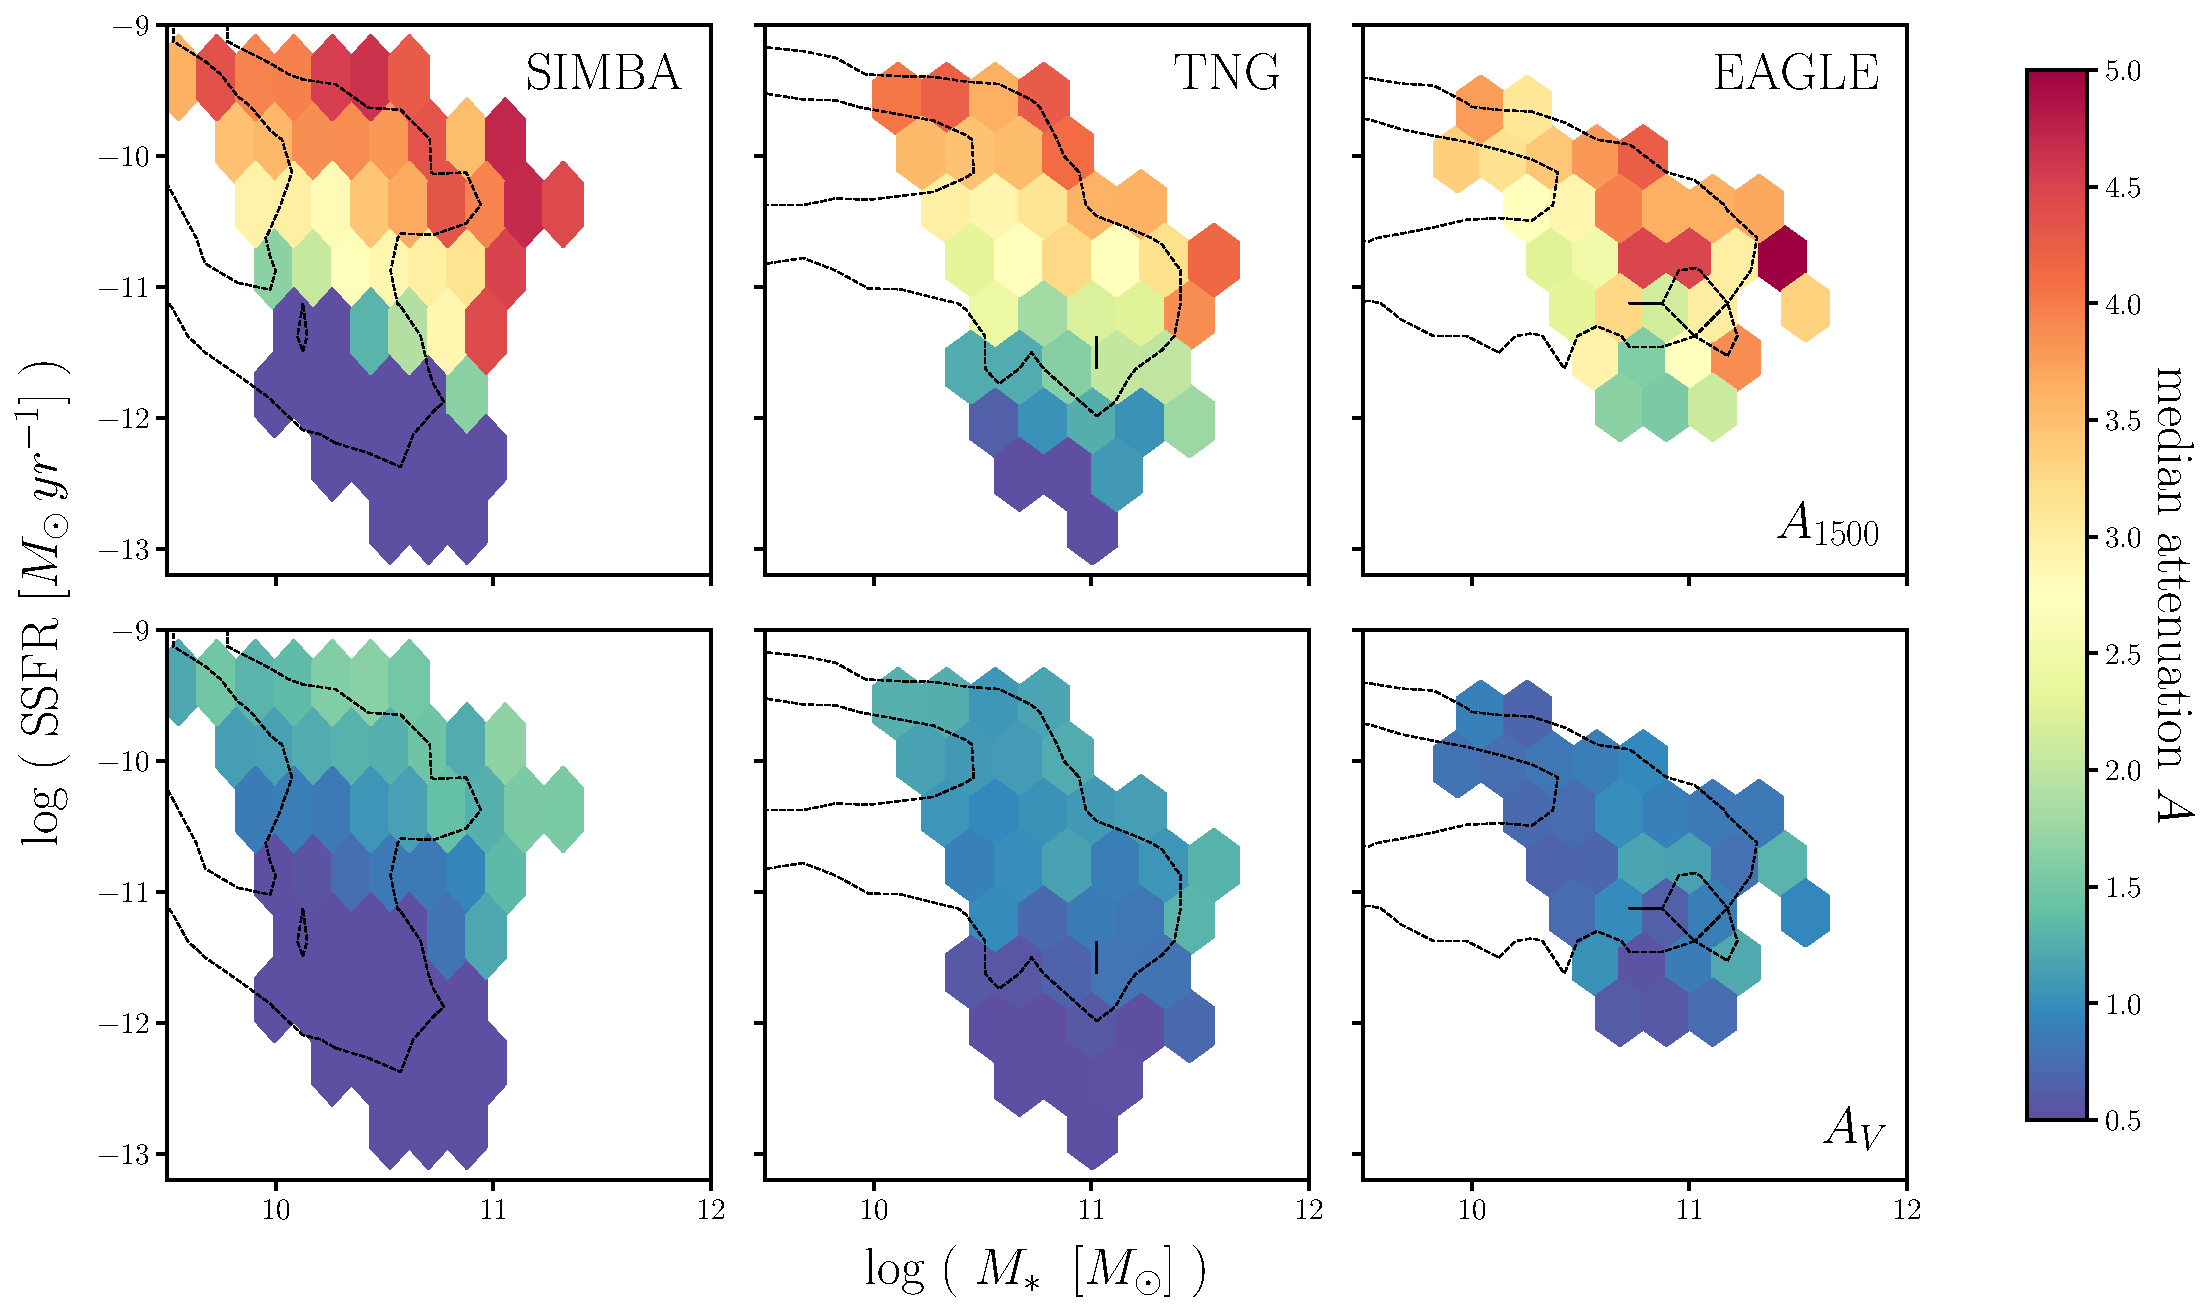
\includegraphics[width=0.9\textwidth]{figs/abc_av_mssfr.pdf}
    \caption{\label{fig:avmsfr}
    }
\end{center}
\end{figure}

\subsection{The Galaxy -- Dust Connection}  
Since the \eda~models predict dust attenuation for all galaxies in the sample,
they allow us to shed light on the
connection between galaxy properties and dust attenuation.  More specifically, 
the \eda~parameters constraints (Figure~\ref{fig:abc}) and the predicted
attenuation curves (Figures~\ref{fig:atten} and~\ref{fig:raw_atten}) reveal the
stellar mass and SSFR dependence of dust attenuation. 
Focusing first on the $M_*$ dependence, we find that TNG has little $M_*$
dependence in $\tau_V$ ($\mtaum = -0.15\substack{+0.83 \\ -0.91}$) while EAGLE
has a significant $M_*$ dependence ($\mtaum = 0.55\substack{+0.40 \\ -0.37}$).
Meanwhile, we find significant $M_*$ dependence in $\delta$ for both TNG 
($\mdeltam = -0.44\substack{+0.27\\-0.26}$) and EAGLE ($\mdeltam =
-0.20\substack{+0.17\\-0.17}$) --- \ie~more massive galaxies have steeper
slopes (Figure~\ref{fig:abc}). The $M_*$ dependence in $\tau_V$ and $\delta$
are further illustrated in the attenuation curves in Figure~\ref{fig:raw_atten}.
For TNG, there is little difference in the $V$-band attenuation between the 
top and bottom panels. However, more massive galaxies have steeper slopes 
with similar $A_V$ so they have significantly higher UV attenuation. For
EAGLE, more massive galaxies have both higher $V$-band and UV attenuation.
Overall, we find that more massive galaxies have higher attenuation,
which is consistent with the literature. \cite{burgarella2005}, for instance,
found significant positive $M_*$ dependence in $FUV$ attenuation in
NUV-selected and FIR-selected samples. \cite{garn2010} and \cite{battisti2016}
also find higher attenuation in more massive SDSS star-forming galaxies. Most
recently, \cite{salim2018} find higher $V$ and $FUV$ attenuation for more
masssive star-forming galaxies in GSWLC2. 

Next, we examine the SSFR dependence of dust attenuation. For both TNG and
EAGLE, we find a significantly negative SSFR dependence in $\tau_V$ 
($\mtaus = -0.56\substack{+0.36 \\ -0.30}$ and
$-0.24\substack{+0.21 \\ -0.20}$, respectively) as well as $\delta$ 
($\mdeltas = -0.57\substack{+0.14 \\ -0.112}$ and $-0.43\substack{+0.10 \\ -0.09}$,
respectively). In other words, galaxies with higher SSFR have lower $V$-band
attenuation and steeper attenuation curves. From the attenuation curves in
Figure~\ref{fig:raw_atten}, we similarly find that star-forming galaxies have
attenuation curves with slightly lower $A_V$ but substantially higher UV 
attenuation. Quiescent galaxies, on the other hand, have significantly 
shallower attenuation curves. Although observations have examined the
SSFR dependence of dust attenuation, they cannot be compared to our findings since
they focus only on star-forming galaxies, due to the difficulty in
observationally constraining the attenuation curve in quiescent
galaxies~\citep[\eg][]{garn2010, reddy2015, battisti2016, battisti2017, salim2018}. 
In summary, from the bestfit \eda~models of TNG and EAGLE, we find that
\emph{galaxies with higher $M_*$ have overall higher dust attenuation and
galaxies with higher SSFR have steeper attenuation curves}.
